\documentclass[journal,12pt,twocolumn]{IEEEtran}

\usepackage{setspace}
\usepackage{gensymb}

\singlespacing


\usepackage[cmex10]{amsmath}

\usepackage{amsthm}

\usepackage{mathrsfs}
\usepackage{txfonts}
\usepackage{stfloats}
\usepackage{bm}
\usepackage{cite}
\usepackage{cases}
\usepackage{subfig}

\usepackage{longtable}
\usepackage{multirow}

\usepackage{enumitem}
\usepackage{mathtools}
\usepackage{steinmetz}
\usepackage{tikz}
\usepackage{circuitikz}
\usepackage{verbatim}
\usepackage{tfrupee}
\usepackage[breaklinks=true]{hyperref}
\usepackage{graphicx}
\usepackage{tkz-euclide}
\usepackage{float}

\usetikzlibrary{calc,math}
\usepackage{listings}
    \usepackage{color}                                            %%
    \usepackage{array}                                            %%
    \usepackage{longtable}                                        %%
    \usepackage{calc}                                             %%
    \usepackage{multirow}                                         %%
    \usepackage{hhline}                                           %%
    \usepackage{ifthen}                                           %%
    \usepackage{lscape}     
\usepackage{multicol}
\usepackage{chngcntr}

\DeclareMathOperator*{\Res}{Res}

\renewcommand\thesection{\arabic{section}}
\renewcommand\thesubsection{\thesection.\arabic{subsection}}
\renewcommand\thesubsubsection{\thesubsection.\arabic{subsubsection}}

\renewcommand\thesectiondis{\arabic{section}}
\renewcommand\thesubsectiondis{\thesectiondis.\arabic{subsection}}
\renewcommand\thesubsubsectiondis{\thesubsectiondis.\arabic{subsubsection}}


\hyphenation{op-tical net-works semi-conduc-tor}
\def\inputGnumericTable{}                                 %%

\lstset{
%language=C,
frame=single, 
breaklines=true,
columns=fullflexible
}
\begin{document}
\newtheorem{theorem}{Theorem}[section]
\newtheorem{problem}{Problem}
\newtheorem{proposition}{Proposition}[section]
\newtheorem{lemma}{Lemma}[section]
\newtheorem{corollary}[theorem]{Corollary}
\newtheorem{example}{Example}[section]
\newtheorem{definition}[problem]{Definition}

\newcommand{\BEQA}{\begin{eqnarray}}
\newcommand{\EEQA}{\end{eqnarray}}
\newcommand{\define}{\stackrel{\triangle}{=}}
\bibliographystyle{IEEEtran}
\providecommand{\mbf}{\mathbf}
\providecommand{\pr}[1]{\ensuremath{\Pr\left(#1\right)}}
\providecommand{\qfunc}[1]{\ensuremath{Q\left(#1\right)}}
\providecommand{\sbrak}[1]{\ensuremath{{}\left[#1\right]}}
\providecommand{\lsbrak}[1]{\ensuremath{{}\left[#1\right.}}
\providecommand{\rsbrak}[1]{\ensuremath{{}\left.#1\right]}}
\providecommand{\brak}[1]{\ensuremath{\left(#1\right)}}
\providecommand{\lbrak}[1]{\ensuremath{\left(#1\right.}}
\providecommand{\rbrak}[1]{\ensuremath{\left.#1\right)}}
\providecommand{\cbrak}[1]{\ensuremath{\left\{#1\right\}}}
\providecommand{\lcbrak}[1]{\ensuremath{\left\{#1\right.}}
\providecommand{\rcbrak}[1]{\ensuremath{\left.#1\right\}}}
\theoremstyle{remark}
\newtheorem{rem}{Remark}
\newcommand{\sgn}{\mathop{\mathrm{sgn}}}
\providecommand{\abs}[1]{\vert#1\vert}
\providecommand{\res}[1]{\Res\displaylimits_{#1}} 
\providecommand{\norm}[1]{\lVert#1\rVert}
%\providecommand{\norm}[1]{\lVert#1\rVert}
\providecommand{\mtx}[1]{\mathbf{#1}}
\providecommand{\mean}[1]{E[ #1 ]}
\providecommand{\fourier}{\overset{\mathcal{F}}{ \rightleftharpoons}}
%\providecommand{\hilbert}{\overset{\mathcal{H}}{ \rightleftharpoons}}
\providecommand{\system}{\overset{\mathcal{H}}{ \longleftrightarrow}}
	%\newcommand{\solution}[2]{\textbf{Solution:}{#1}}
\newcommand{\solution}{\noindent \textbf{Solution: }}
\newcommand{\cosec}{\,\text{cosec}\,}
\providecommand{\dec}[2]{\ensuremath{\overset{#1}{\underset{#2}{\gtrless}}}}
\newcommand{\myvec}[1]{\ensuremath{\begin{pmatrix}#1\end{pmatrix}}}
\newcommand{\mydet}[1]{\ensuremath{\begin{vmatrix}#1\end{vmatrix}}}
\numberwithin{equation}{subsection}
\makeatletter
\@addtoreset{figure}{problem}
\makeatother
\let\StandardTheFigure\thefigure
\let\vec\mathbf
\renewcommand{\thefigure}{\theproblem}
\def\putbox#1#2#3{\makebox[0in][l]{\makebox[#1][l]{}\raisebox{\baselineskip}[0in][0in]{\raisebox{#2}[0in][0in]{#3}}}}
     \def\rightbox#1{\makebox[0in][r]{#1}}
     \def\centbox#1{\makebox[0in]{#1}}
     \def\topbox#1{\raisebox{-\baselineskip}[0in][0in]{#1}}
     \def\midbox#1{\raisebox{-0.5\baselineskip}[0in][0in]{#1}}
\vspace{3cm}
\title{Assignment 5}
\author{Dhatri Nanda \\ AI20BTECH11002}
\maketitle
\newpage
\bigskip
\renewcommand{\thefigure}{\theenumi}
\renewcommand{\thetable}{\theenumi}
Download all python codes from 
\begin{lstlisting}
https://github.com/Dhatri-nanda/EE3900/blob/main/Assignment_5/code.py
\end{lstlisting}
%
and latex-tikz codes from 
%
\begin{lstlisting}
https://github.com/Dhatri-nanda/EE3900/blob/main/Assignment_5/Assignment_5.tex
\end{lstlisting}
\section{Quadratic Forms 2.37}
Prove that the parabolas $y^2 = 4x$ and $x^2 = 4y$ divide the area of the square bounded by $x=0$, $x=4$, $y=4$ and $y=0$ into three equal parts

\section{Solution}
\begin{lemma}
The points of intersection of \textbf{Line} $L:\vec{x}=\vec{q}+\mu\vec{m}$ with \textbf{parabola}

\begin{align}
\vec{x^T}\vec{V}\vec{x}+2\vec{u^T}\vec{x}+f=0
\end{align}

is given by:
\begin{align}
\vec{x}_i = \vec{q}+\mu_i\vec{m}
\end{align}
%
where,
\begin{multline}
\mu_i = \frac{1}
{
\vec{m}^T\vec{V}\vec{m}
}
\lbrak{-\vec{m}^T\brak{\vec{V}\vec{q}+\vec{u}}}
\\
\pm
{\small
\rbrak{\sqrt{
\sbrak{
\vec{m}^T\brak{\vec{V}\vec{q}+\vec{u}}
}^2
-
\brak
{
\vec{q}^T\vec{V}\vec{q} + 2\vec{u}^T\vec{q} +f
}
\brak{\vec{m}^T\vec{V}\vec{m}}
}
}
}\label{quad}
\end{multline}
\end{lemma}
\begin{proof}
The points of intersection must satisfy the line and parabola equation.
Thus,
\begin{align}
\vec{\brak{\vec{q}+\mu\vec{m}}^T}\vec{V}\vec{\brak{\vec{q}+ \mu\vec{m}}}+2\vec{u^T}\vec{\brak{\vec{q}+\mu\vec{m}}}+f=0
\end{align}
On expansion, we get
\begin{multline}
  \mu^2\vec{m^T}\vec{V}\vec{m}+ \mu\sbrak{\vec{m^T}\vec{V}\vec{q}+\vec{q^T}\vec{V}\vec{m}+2\vec{u^T}\vec{m}}\\ + \vec{q^T}\vec{V}\vec{q}+2\vec{u^T}\vec{m}+f=0  
\end{multline}
Since, $\vec{q^T}\vec{V}\vec{m},2\vec{u^T}\vec{m}$ are scalars
\begin{align}
 \vec{q^T}\vec{V}\vec{m}=\vec{m^T}\vec{V^T}\vec{q} \\
 2\vec{u^T}\vec{m}=2\vec{m^T}\vec{u}
\end{align}
Solving the above quadratic equation we get
\begin{multline}
\mu_i = \frac{1}
{\vec{m}^T\vec{V}\vec{m}
}\lbrak{-\vec{m}^T\brak{\vec{V}\vec{q}+\vec{u}}}
\\\pm{\small
\rbrak{\sqrt{
\sbrak{
\vec{m}^T\brak{\vec{V}\vec{q}+\vec{u}}
}^2-\brak{\vec{q}^T\vec{V}\vec{q} + 2\vec{u}^T\vec{q} +f
}\brak{\vec{m}^T\vec{V}\vec{m}}
}}}
\end{multline}
\end{proof}
\textbf{First} we consider the parabola $x^2 = 4y$

The matrix parameters of the parabola are
\begin{align}
\vec{V}=\myvec{1&0\\0&0},\vec{u}=\myvec{0\\-2},f=0 \label{quadform/2/105/eq:v}
\end{align}

Now, we find the points of intersections with the square

The first line is
\begin{align} 
y=4
\end{align}

 The parametric form is:
\begin{align} 
L: \vec{x}&=\vec{q}+\mu\vec{m}
\\
\implies \vec{x}&=\myvec{0\\4}+\mu\myvec{1\\0} \label{quadform/2/105/eq:q}
\end{align}
From  \eqref{quad},
\begin{align}
\mu_1 &= 4, \mu_2 =-4
\end{align}
Substituting $\mu_1$ and $\mu_2$ in \eqref{quadform/2/105/eq:q},the points of intersection
\begin{align}
 \vec{M_1}= \myvec{4\\4},  
\vec{P_1}&= \myvec{-4\\4}
\end{align}

The next line is 
\begin{align} 
y=0
\end{align}
The parametric form is:
\begin{align} 
L: \vec{x}&=\vec{q}+\mu\vec{m}
\\
\implies \vec{x}&=\myvec{0\\0}+\mu\myvec{1\\0} \label{quadform/2/105/eq:r}
\end{align}
From  \eqref{quad},
\begin{align}
\mu = 0
\end{align}
Substituting $\mu$ in \eqref{quadform/2/105/eq:r},the point of intersection
\begin{align}
 \vec{K_1}= \myvec{0\\0}
\end{align}

\textbf{Next} we consider the parabola $y^2 = 4x$

The matrix parameters of the parabola are
\begin{align}
\vec{V}=\myvec{0&0\\0&1},\vec{u}=\myvec{-2\\0},f=0 \label{quadform/2/105/eq:vi}
\end{align}


The first line is
\begin{align} 
y=4
\end{align}

 The parametric form is:
\begin{align} 
L: \vec{x}&=\vec{q}+\mu\vec{m}
\\
\implies \vec{x}&=\myvec{0\\4}+\mu\myvec{1\\0} \label{quadform/2/105/eq:qi}
\end{align}
From  \eqref{quad},
\begin{align}
\mu &= 4
\end{align}
Substituting $\mu$ in \eqref{quadform/2/105/eq:qi},the points of intersection
\begin{align}
 \vec{M_2}= \myvec{4\\4}
\end{align}

The next line is 
\begin{align} 
y=0
\end{align}
The parametric form is:
\begin{align} 
L: \vec{x}&=\vec{q}+\mu\vec{m}
\\
\implies \vec{x}&=\myvec{0\\0}+\mu\myvec{1\\0} \label{quadform/2/105/eq:ri}
\end{align}
From  \eqref{quad},
\begin{align}
\mu = 0
\end{align}
Substituting $\mu$ in \eqref{quadform/2/105/eq:ri},the point of intersection
\begin{align}
 \vec{K_2}= \myvec{0\\0}
\end{align}

So, both the parabolas intersect each other and the given square at the points 
\begin{align}
 \vec{K}= \myvec{0\\0},
 \vec{M}= \myvec{4\\4}
\end{align}


Area of the square i.e., $A_1$ 
\begin{align}
    A_1 &= Ar(KLMNK)\\
    &= \int_0^4 4dx\\
    &= 16
\end{align}

Area under the parabola $y^2 = 4x$ i.e., $A_2$
\begin{align}
    A_2 &= \int_0^4 \sqrt{4x} dx\\
   &= \frac{1}{6}((16)^{3/2} - 0)\\
   &= \frac{32}{3}
\end{align}

Area under the parabola $x^2 = 4y$ i.e., $A_3$
\begin{align}
    A_3 &= \int_0^4 \frac{x^2}{4}\\
    &= \frac{1}{12}((4)^3 - 0)\\
    &= \frac{16}{3}
\end{align}
As shown in the figure, as the parabolas divide the square into 3 parts

Area of first region is
\begin{align}
    A &= A_1 - A_2\\
    &= 16 - \frac{32}{3} \\
    &= \frac{16}{3}
\end{align}

Area of the second region is
\begin{align}
    B &= A_2 - A_3\\
    &= \frac{32}{3} - \frac{16}{3}\\
    &= \frac{16}{3}
\end{align}

Area of the third region is
\begin{align}
    C &= A_3\\
    &= \frac{16}{3}
\end{align}

So, the 2 parabolas divide the area bounded by the square into 3 equal parts.
\begin{figure}[ht]
\centering
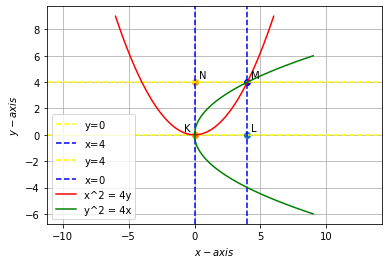
\includegraphics[width=\columnwidth]{AS_5.png}
\caption{plot}
\label{fig:my_label}
\end{figure}
\end{document}